\documentclass[11pt,letterpaper]{article}

% Essential packages
\usepackage[utf8]{inputenc}
\usepackage[english]{babel}
\usepackage{amsmath,amssymb,amsfonts}
\usepackage{graphicx}
\usepackage{float}
\usepackage{hyperref}
\usepackage{geometry}

% Page layout
\geometry{
    letterpaper,
    margin=1in
}

% Hyperlink colors
\hypersetup{
    colorlinks=true,
    linkcolor=blue,
    filecolor=magenta,      
    urlcolor=cyan,
}

\begin{document}

% Simple header with student name
\begin{center}
    {\Large\bfseries Final Competition Report\par}
    \vspace{0.3cm}
    {\large ENAE450 - Robotics Programming\par}
    \vspace{0.5cm}
\end{center}

\noindent
\textbf{Student Names:} {Conner Davidsen, Brian Fugh, Akash Wudali, Pranavsai Akurati}

\noindent
\textbf{Date:} \today

\vspace{0.5cm}

\section{Introduction}

The final competition for ENAE450: Robotics Programming consists of navigating a maze from a start to end zone using the turtlebot 4. We do this by deploying a fully autonomous ROS 2 stack that allows the turtlebot to navigate the maze. 
We will complete two different maze races. The first is a pre-mapping race where we scan the maze and give it to the robot


\section{Hardware: Methods and Results}

\section{Competition Runs}

% replace images with turtlebot plot during run
\begin{figure}[H]
    \centering
    % Replace 'screenshot_placeholder.png' with your actual screenshot filename (screenshot.png)
    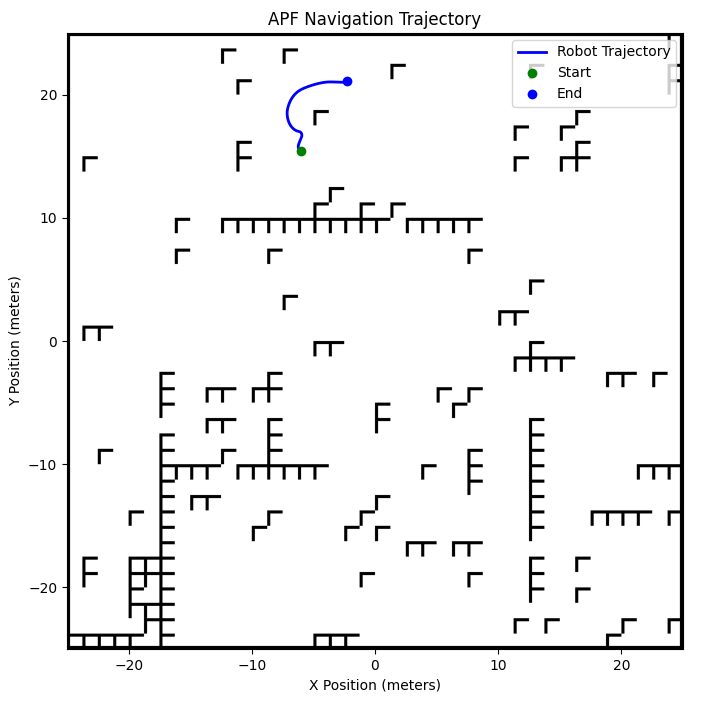
\includegraphics[width=0.9\textwidth]{navigation_path.png}
    \caption{Turtlebot trajectory of attractive + repulsive potential field navigation }
    \label{fig:path_trajectory}
\end{figure}

\section{Retrospective}

\section{Contributions}



\section*{References}

% Add additional references as needed/practical
\begin{itemize}
    \item ROS2 Documentation: \url{https://docs.ros.org}
\end{itemize}

\end{document}
